\chapter{Implementacja}
\vspace{-20pt}

Rozdział ten opisuje w jaki sposób zostały zrealizowane założenia projektu z podziałem na poszczególne pliki. Przedstawia również dokładnie i szczegółowo opisane rozwiązania implementacyjne zadań, na które projekt został podzielony.

\section{Odebranie sygnału wyjściowego z keyboardu i zapis}

\noindent\textbf{midi.py}

Odpowiada za znalezienie odpowiedniego urządzenia spośród wejściowych portów, odbieranie sygnału muzycznego oraz za zapis do zmiennej odbieranego sygnału przez ustalony czas.

Z użyciem biblioteki Pygame \cite{pygame} zostaje znaleziona ilość portów i sprawdza podłączone do nich urządzenia. Wybiera właściwe oraz wybiera sygnał wyjściowy urządzenia. Gdy takowe nie zostanie znalezione, zwraca komunikat o nieznalezieniu żadnego wejścia midi. Natomiast jeśli zostanie znalezione, tworzy macierz za pomocą biblioteki NumPy \cite{numpy} o rozmiarze skali dwunastotonowej na 10, czyli ilość oktaw obejmującą zakres częstotliwości zawierający częstotliwości praktycznie wszystkich instrumentów muzycznych. Macierz ta służy do zapisu czasu wciśnięcia konkretnego klawisza, ze względu na charakterystykę przychodzenia sygnału z keyboardu, a mianowicie dostarczaniu sygnału po wciśnięciu klawisza oraz po jego odpuszczeniu, natomiast czas jest naliczany za pomocą Pygame \cite{pygame}. Sygnał był odbierany przez czas, określony w zależności od potrzeb. Zawiera informacje dotyczące kanału, z którego pochodzi dźwięk, nutę, amplitudę, czas oraz interakcje z klawiszem. Następnie tak jak w formacie midi zapisywana jest akcja o wciśnięciu konkretnych klawiszy i czas oraz potem o ich odpuszczeniu.\\

\noindent\textbf{midisave.py}

Służy do zapisu uprzednio zebranego sygnału do pliku w formacie midi.
Uruchamia plik midi.py, z którego odebranej sekwencji czas jest przeliczany z bezwzględnego na względny względem siebie, tak jak odczytuje to format midi. Za pomocą biblioteki Mido \cite{mido} ta kombinacja jest konwertowana i zapisywana jako plik w formacie midi.\\

\newpage
\noindent\textbf{miditomp3.py}

Użycie FluidSynth \cite{fluidsynth} i biblioteki midi2audio \cite{midi2audio} pozwoliło zmienić uzyskany wcześniej plik midi na plik w formacie mp3 z użyciem dowolnie wybranego soundfontu, a zatem metody syntezy wavetable.\\

Użycie powyższych skryptów umożliwiło pozyskanie pliku z własnej gry, a co za tym idzie testowanie własnoręcznie zagranych sekwencji, a zarazem dokładniejsze zrozumienie cech dźwięku i sprawdzenie działania reszty programu.

\section{Uzyskanie spektrogramu przy użyciu transformaty Fouriera}

\noindent\textbf{fourier.py}

Ten element odpowiada za utworzenie widma wybranego pliku audio. Z użyciem biblioteki os odczytywana jest ścieżka do wybranego pliku, a następnie za pomocą biblioteki LibROSA \cite{librosa} ze wskazanego pliku odczytywana jest częstotliwość próbkowania oraz wektor reprezentujący amplitudę całego sygnału audio. Następnie określona wartość  $n\_fft$ wynoszące $2^{14}$ i $hop\_length$ wynoszące $2^8$. Wartości te oznaczają odpowiednio liczbę punktów próbkowania użytych do każdej ramki oraz ilość próbek między kolejnymi ramkami.

W dalszym kroku za pomocą funkcji librosa.stft obliczana jest transformata Fouriera z wczytanego uprzednio sygnału audio i ustalonych wartości, czego efektem końcowym jest uzyskanie macierzy amplitud. Następuje konwersja na decybele i zostaje wyświetlony oraz zapisany za pomocą biblioteki Matplotlib \cite{matplotlib} wykres powstałego widma, gdzie oś x reprezentuje czas, oś y częstotliwości, a natężenie koloru odpowiada za głośność.

\section{ Analiza uzyskanego widma i konwersja na plik w formacie midi}

\noindent\textbf{spektrummidi.py}

Użycie pliku fourier.py pozwala na przekształcenie widma ścieżki dźwiękowej za pomocą algorytmu na format muzyczny midi. 
Algorytm ten na początek otrzymuje widmo pliku audio w postaci macierzy amplitud oraz wektor częstotliwości i wektor czasu. Zawarta lista z częstotliwościami odpowiadającymi danym tonom (Tab. 2.1) jest porównywana do częstotliwości otrzymanych ze skryptu fourier.py i zostają zapisane indeksy częstotliwości, które są najbliżej częstotliwości szukanych. Lista ta została zmodyfikowana, użyte zostały częstotliwości z najwyższej oktawy, a następnie kolejno dzielone przez 2, aby uzyskać dokładniejsze niższe częstotliwości. Porównywanie polega na przechodzeniu po wszystkich częstotliwościach z tabeli, których jest 12 dźwięków przez 9 oktaw, czyli 108, a następnie po wszystkich częstotliwościach z użycia transformaty Fouriera sprawdzając po kolei, dla której wartości bezwzględna różnica będzie najmniejsza. 	
Po uzyskaniu indeksów pożądanych częstotliwości z widma może się odbyć przeszukiwanie macierzy amplitud po tych częstotliwościach. Nim ten proces się rozpocznie, zostaje znaleziona wartość maksymalna występującej amplitudy, a następnie z użyciem biblioteki NumPy \cite{numpy} tworzona jest lista list, do której zapisywane będą znalezione przez algorytm dominujące dźwięki. Sam algorytm zaś przeszukuje każdy ton po czasie tak jak to zostało opisane w podrozdziale 3.3. Algorytm.
Po przeszukaniu całego sygnału, uzyskane wartości zostają zapisane za pomocą skryptu midisave.py, co pozwala na odtworzenie wyniku końcowego.

\section{Powstawanie synthesii ze ścieżki audio w formacie midi}

\noindent\textbf{openmidi.py}

Po wskazaniu ścieżki audio następuje przekształcenie wybranej piosenki z formatu midi za pomocą biblioteki mido \cite{mido} na listę słowników.\\

\noindent\textbf{graphic.py}

Główny skrypt odpowiadający za wyświetlanie synthesii rozpoczyna działanie od zdefiniowania funkcji. 

Funkcja \_\_init\_\_() rozpoczyna się inicjalizacją wszystkich modułów dostarczanych przez bibliotekę Pygame \cite{pygame}. Następnie zostają zebrane i ustawione dane o rozdzielczości monitora, dodane flagi ustawiające pełny ekran i podwójne buforowanie, co wspomaga optymalizację. Natomiast druga funkcja run() zawiera w sobie główną pętlę, która odpowiada za obliczanie i wyświetlanie oraz zawiera w sobie dwie funkcje zagnieżdżone.

Funkcja convert\_song() odpowiada za przekonwertowanie listy zawierającej akcje dotyczące każdego pojedynczego tonu. Konwersja polega na połączeniu akcji rozpoczęcia trwania tonu i akcji jego zakończenia na ton, który zawiera czas trwania. Konwersja powoduje również zmianę z czasu względnego, jaki występuje w formacie midi, na czas bezwzględny. Po tym następuje sortowanie tonów względem czasu i zwrócone w postaci listy do wyświetlenia. Natomiast zadaniem drugiej funkcji key\_parametres() jest przekształcenie tonu na klawisz, zwracając jego miejsce położenia, szerokość oraz kolor, dla półtonów czarny i dla pełnych tonów biały.

Funkcja player\_info sprawdza, czy istnieje plik tekstowy z danymi gracza. Jeśli tak to sprawdza, czy zawiera informacje o ilości punktów uprzednio zgromadzonych przez gracza. Jeśli nie to tworzy plik tekstowy o nazwie uprzednio podanej przez gracza.

\newpage
Kolejnym krokiem jest przygotowanie zmiennych używanych w głównej pętli. Zależnie od ilości oktaw i szerokości ekranu odpowiednio wyliczana jest szerokość białych klawiszy.

\begin{equation}
\[
w = \frac{s}{7 \cdot o}
\]
\end{equation}

gdzie:
\begin{itemize}
    \item \(w\) jest szerokością białego klawisza,
    \item \(s\) jest szerokością ekranu,
    \item \(o\) jest liczbą oktaw.
\end{itemize}

Następnie na podstawie pliku midi.py zostaje przechwycony sygnał z keyboardu, co pozwala na porównywanie gry użytkownika względem włączonej piosenki. Najważniejszą częścią jest główna pętla, która rozpoczyna się od jednorazowego utworzenia całej klawiatury. Najpierw są tworzone białe klawisze, następnie czarne po wszystkich oktawach. 

\begin{figure}[h]
  \centering
  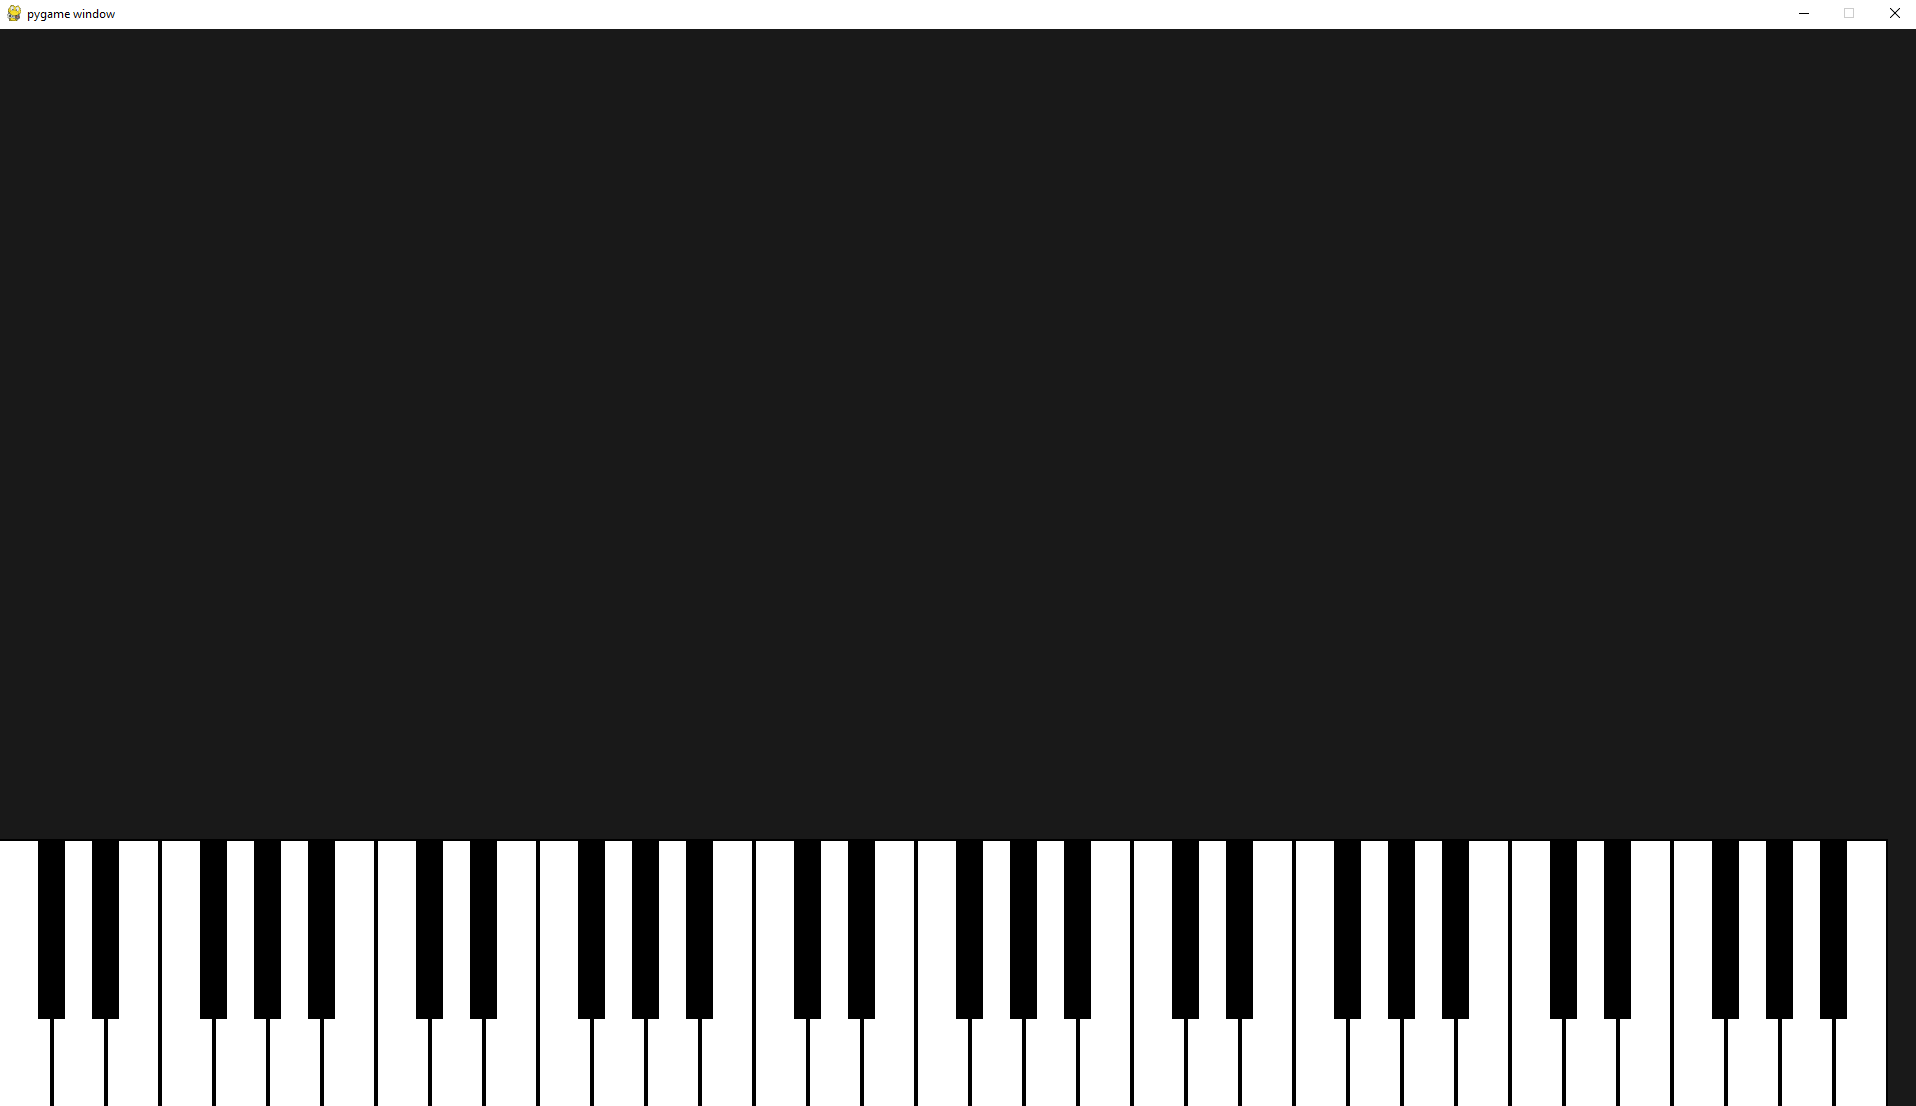
\includegraphics[width=1\textwidth]{img/4/klawiatura.png}
  \caption{Wygląd rozpoczętej gry}
\end{figure}

W kolejnym kroku program sprawdza, czy przyszedł sygnał pochodzący z interakcji użytkownika z keyboardem. Potem następuje część odpowiedzialna za wyświetlanie całego utworu muzycznego. Porównując czas pierwszego tonu w liście z aktualnym, jest on usuwany z aktualnej i przenoszony do listy wyświetlanych tonów.

Następnie pętla przechodząca po tejże liście oblicza wysokość na ekranie każdego tonu ograniczając go, aby na początku nie był widoczny na ekranie, a na wysokości rozpoczynania się klawiatury został usunięty z listy wyświetlanych tonów. Długość natomiast początkowo jest proporcjonalna do czasu trwania tonu, a gdy ma zacząć zakrywać klawiaturę, jest adekwatnie zmniejszana. W tym samym momencie zaczyna się podświetlać klawisz, który użytkownik powinien nacisnąć, a gdy wygasa, część klawiatury podświetlanego klawisza zostaje nadbudowana. Kolejna część jest odpowiedzialna za wyświetlanie synthesii z użyciem pygame.draw.rect, co pozwala na wyświetlenie prostokątnego kształtu z zadanym wcześniej kolorem, szerokością, długością oraz położeniem. Szerokość wyświetlanego kształtu jest zależna od tego, czy to półton czy cały ton oraz szerokość położenia na ekranie zależna od wysokości tonu. Końcówka wyświetlanego tonu zostaje nadbudowywana kolorem tła, aby po jego zakończeniu nie został po nim widoczny ślad, który przeszkadzałby w rozczytywaniu kolejnych tonów.

\begin{figure}[h]
  \centering
  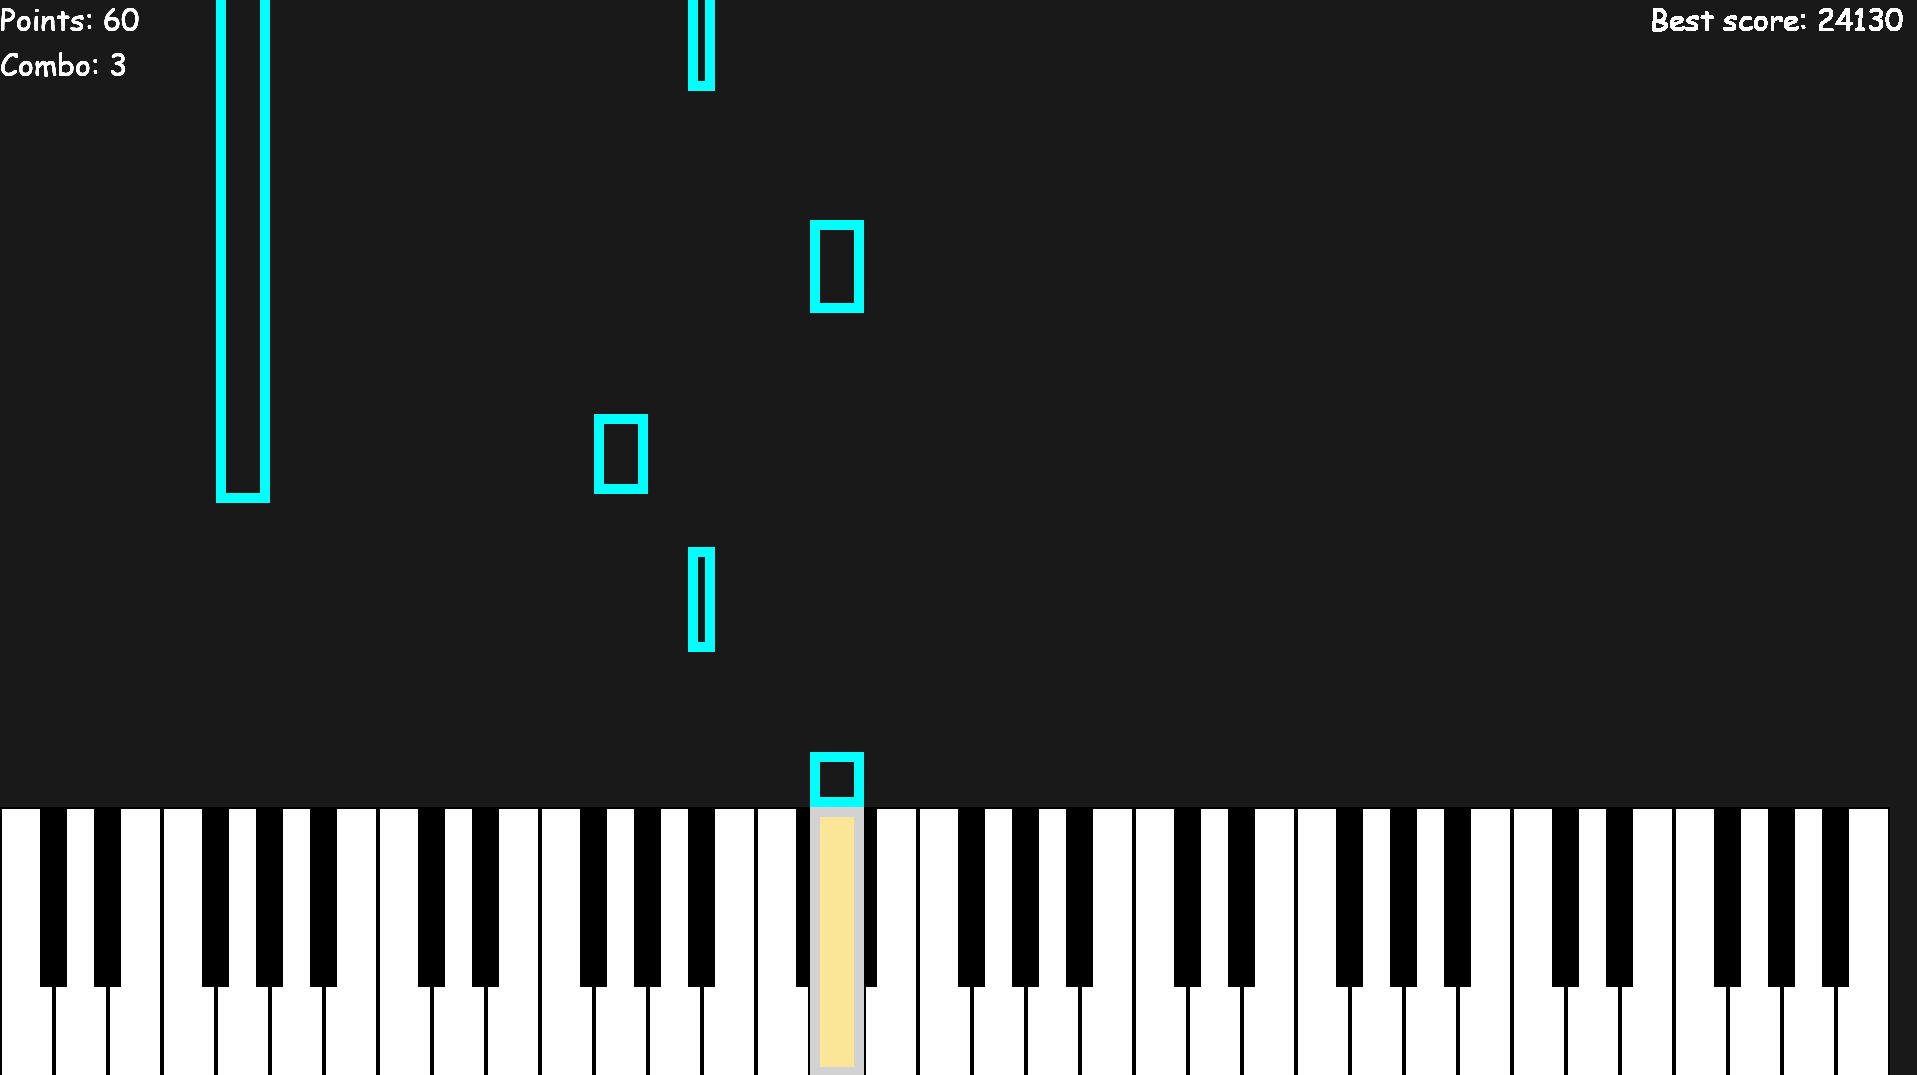
\includegraphics[width=1\textwidth]{img/4/synthesia.png}
  \caption{Wyświetlająca się synthesia}
\end{figure}

Ostatnią częścią dotyczącą synthesii jest zliczanie punktów za poprawne powtarzanie sekwencji na instrumencie. Gdy dany klawisz się podświetla i użytkownik naciśnie go w odpowiednim czasie, zostaną dodane punkty przemnożone przez mnożnik zwiększający się o 1 za każdym poprawnym naciśnięciem oraz zerujący się, gdy któryś klawisz nie zostanie wciśnięty, bądź zostanie naciśnięty nieprawidłowy klawisz. Naliczane punkty są na bieżąco wyświetlane w lewym górnym rogu ekranu gry  (por. Rys. 4.2), a w prawym górnym rogu widnieje najlepszy wynik uzyskany uprzednio przez gracza.

Główna pętla kończy się dodaną funkcjonalnością klawiszy, które pozwalają na rozpoczęcie wyświetlania synthesii oraz na wyjście z niej. Przy opuszczeniu programu, jeśli gracz uzyskał więcej punktów niż swój rekord, bądź nie posiadał jeszcze wyniku dla danej piosenki, ilość zebranych punktów zostaje zapisana do pliku profilu gracza.

\begin{figure}[h]
  \centering
  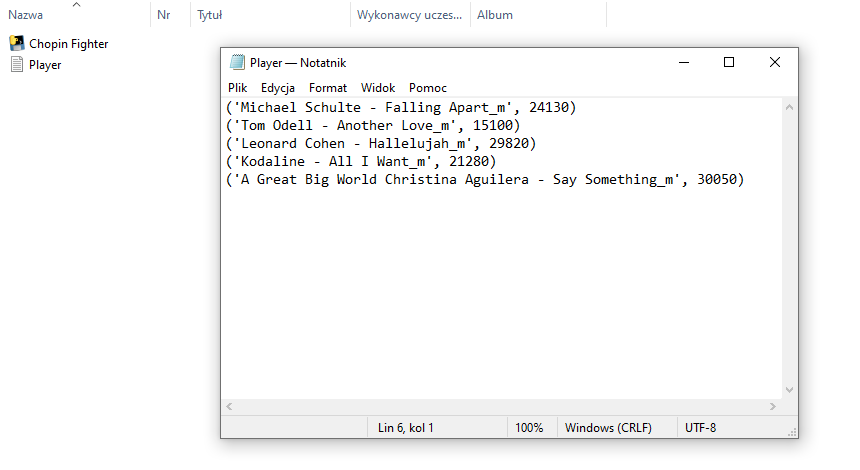
\includegraphics[width=1\textwidth]{img/4/wyniki.png}
  \caption{Stworzony plik z profilem gracza zawierający informacje o najlepszych wynikach}
\end{figure}

\section{Scalenie projektu}

\noindent\textbf{menu.py}

Do scalenia wszystkich plików ważnym elementem było stworzenie funkcjonalnego menu, które będzie zarazem estetyczne i przyjemne dla oka.
Niezbędne okazały się biblioteki Pygame \cite{pygame} oraz pygame-menu \cite{pygame_menu}. Program zawiera w sobie kilka funkcji, które poprzedza zainicjowanie użycia wcześniej wymienionych bibliotek. Na sam początek zostaje zebrana informacja o rozdzielczości ekranu, a następnie utworzone całe menu.

\begin{figure}[h]
  \centering
  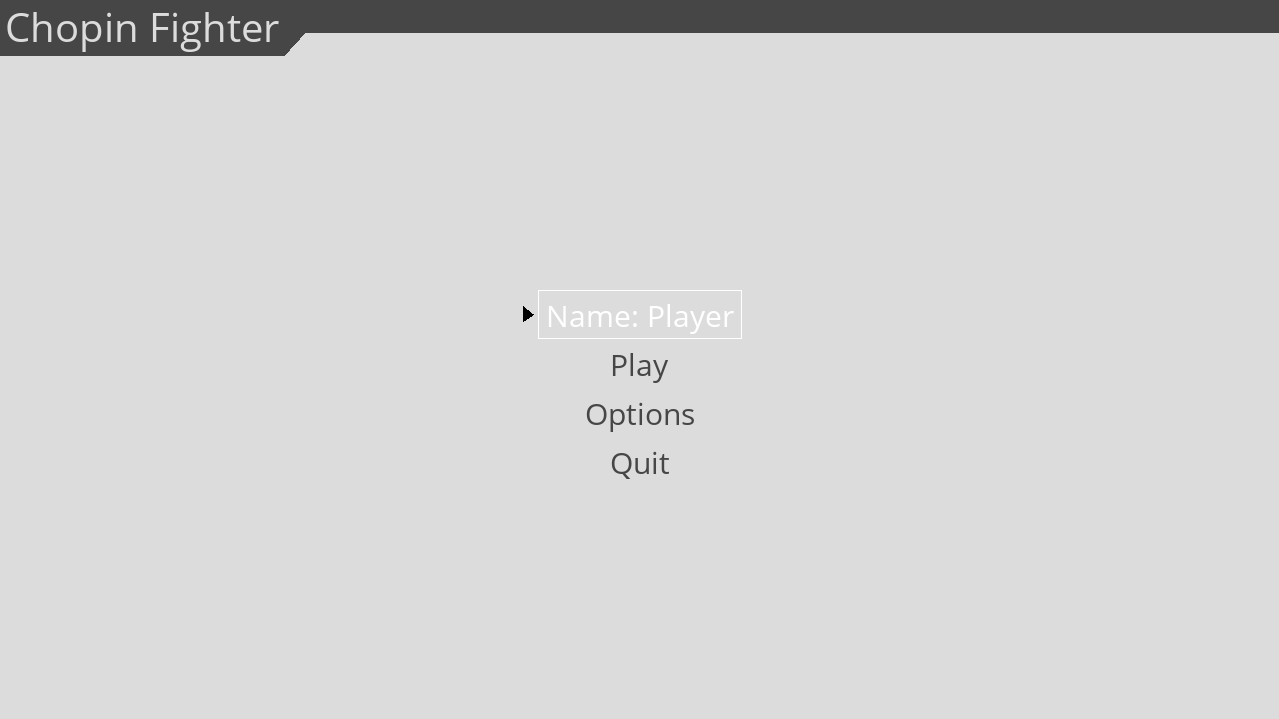
\includegraphics[width=0.88\textwidth]{img/4/menu.png}
  \caption{Menu gotowego programu}
\end{figure}

W głównej pętli menu zbierane są informacje o akcji użytkownika oraz odświeżanie grafiki, przez co menu staje się funkcjonalne. Na początkowym ekranie (por. Rys. 4.4.) widnieją trzy przyciski. Przycisk Quit uruchamia funkcję zatrzymującą główną pętlę oraz kończącą proces biblioteki Pygame \cite{pygame}. Przycisk Options otwiera menu opcji, w którym jest do wyboru rozdzielczość, w jakiej program ma działać. Wybór jest możliwy spośród najczęściej występujących rozdzielczości oraz nominalnej wykrytej na początku. Menu opcji daje możliwość wyboru trudności granego utworu, lecz jest to funkcja koncepcyjna. Wyjść bez zmiany ustawień można przyciskiem w prawym górnym rogu.

\begin{figure}[h]
  \centering
  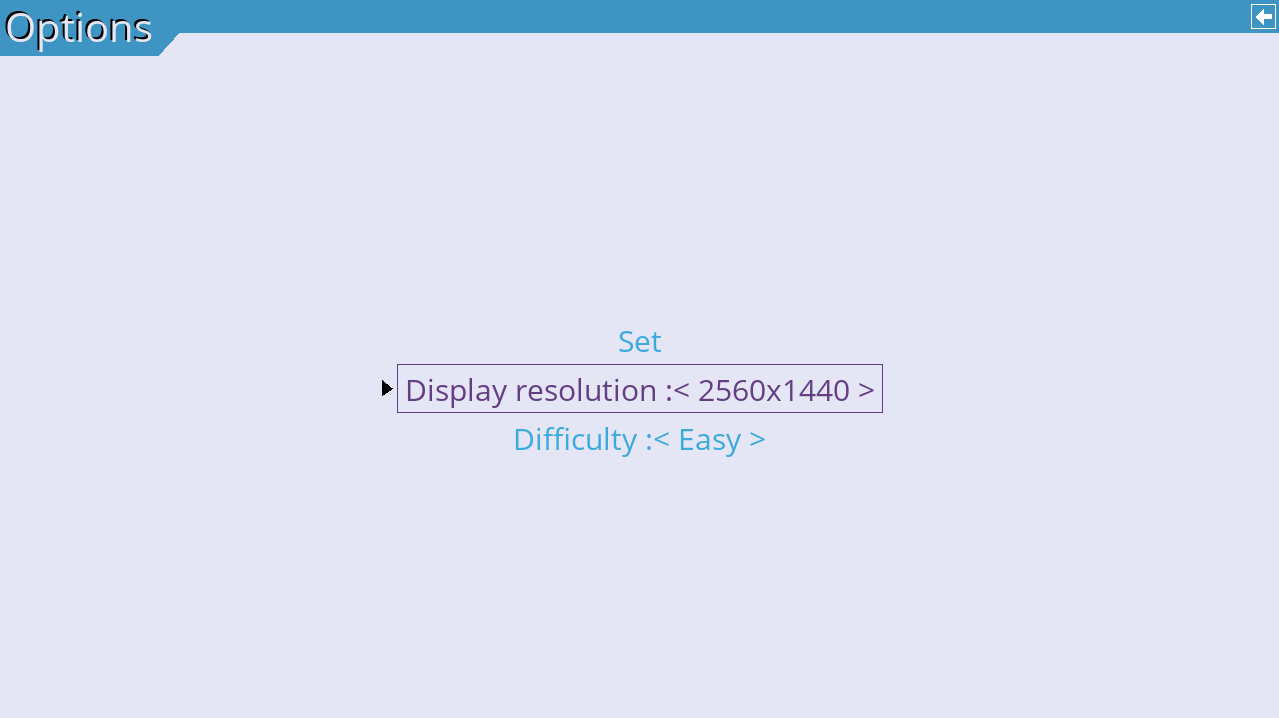
\includegraphics[width=0.88\textwidth]{img/4/opcje.png}
  \caption{Menu opcji}
\end{figure}

\newpage
Przycisk Play powoduje otwarcie się okna do wyboru pliku muzycznego, który w zależności od rozszerzenia pliku uruchomi wyświetlanie synthesii albo analizę pliku muzycznego, a następnie konwersję na format midi, po której dopiero nastąpi wyświetlenie synthesii.

\begin{figure}[h]
  \centering
  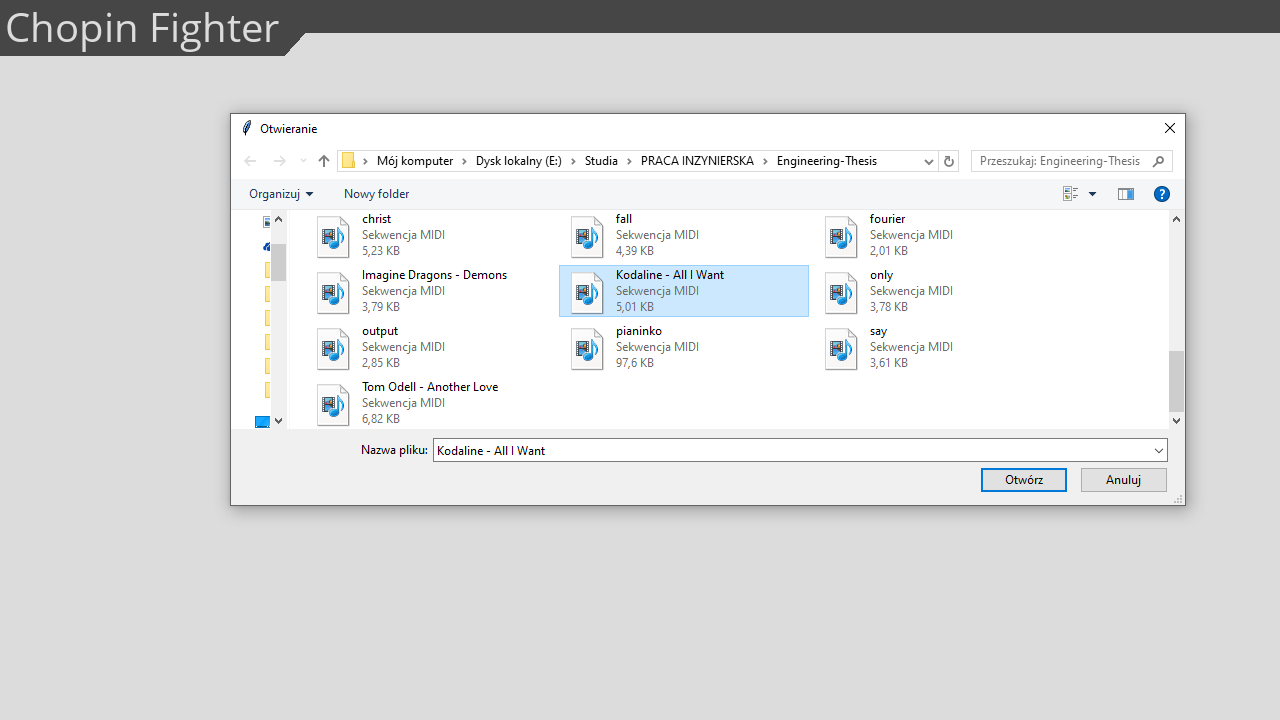
\includegraphics[width=1\textwidth]{img/4/wybor.png}
  \caption{Wybór pliku audio}
\end{figure}